%%%%%%%%%%%%%%%%%%%%%%%%%%%%%%%%%%%%%%%%%%%%%%%%%%%%%%%%%%%%%%%%%%%%%%%%%%%
%%
%% Copyright (c) 2014 Adobe Systems Incorporated. All rights reserved.
%%
%% Licensed under the Apache License, Version 2.0 (the "License");
%% you may not use this file except in compliance with the License.
%% You may obtain a copy of the License at
%%
%% http://www.apache.org/licenses/LICENSE-2.0
%%
%% Unless required by applicable law or agreed to in writing, software
%% distributed under the License is distributed on an "AS IS" BASIS,
%% WITHOUT WARRANTIES OR CONDITIONS OF ANY KIND, either express or implied.
%% See the License for the specific language governing permissions and
%% limitations under the License.
%%
%%%%%%%%%%%%%%%%%%%%%%%%%%%%%%%%%%%%%%%%%%%%%%%%%%%%%%%%%%%%%%%%%%%%%%%%%%%
\documentclass{beamer}
% Theme Matrix: http://www.hartwork.org/beamer-theme-matrix/
%% \mode<presentation> { \usetheme{Malmoe}\usecolortheme{dove} }
\mode<presentation> { \usetheme{Goettingen}\usecolortheme{dove} }
\setbeamertemplate{itemize items}[default]
\usepackage[T1]{fontenc}
\usepackage{parskip,graphics,tikz,multimedia,hyperref,ulem,multicol}
\usepackage{array,multirow}
\usetikzlibrary{arrows,positioning,shapes,decorations.pathmorphing,
  decorations.markings}
\setlength{\itemsep}{0pt}\setlength{\parskip}{0pt}\setlength{\parsep}{0pt}
\graphicspath{{./images/}}

\usepackage{listings,textcomp,color}
\lstset{language=Python,upquote=true,
  basicstyle=\ttfamily\tiny,numbers=left,
  numberstyle=\tiny,stepnumber=1,numbersep=5pt,
  backgroundcolor=\color{white},frame=single,tabsize=2,
  showspaces=false,showstringspaces=false,showtabs=false,
  breaklines=true,breakatwhitespace=true,escapeinside=||,
  keywordstyle=\color{blue!70},stringstyle=\color{green!70!black!70},
  commentstyle=\color{black!80}\it
}
\lstdefinelanguage{scala}{
  morekeywords={abstract,case,catch,class,def,%
    do,else,extends,false,final,finally,%
    for,if,implicit,import,match,mixin,%
    new,null,object,override,package,%
    private,protected,requires,return,sealed,%
    super,this,throw,trait,true,try,%
    type,val,var,while,with,yield},
  otherkeywords={=>,<-,<\%,<:,>:,\#,@},
  sensitive=true,
  morecomment=[l]{//},
  morecomment=[n]{/*}{*/},
  morestring=[b]",
  morestring=[b]',
  morestring=[b]"""
}

%% \usebackgroundtemplate{
%%   \tikz[overlay,remember picture]
%%   \node[yshift=10mm,anchor=south east,inner sep=0pt]
%%     at (current page.south west) {
%%     \includegraphics[width=0.5in]{logo}
%%   };
%% }

\tikzset{
  yn/.style={draw,thick,rounded corners,fill=yellow!20,inner sep=.3cm},
  bn/.style={draw,thick,rounded corners,fill=blue!05,inner sep=.3cm},
  on/.style={draw,thick,rounded corners,fill=orange!20,inner sep=.3cm},
  rn/.style={draw,thick,rounded corners,fill=red!20,inner sep=.3cm},
  wn/.style={draw,thick,rounded corners,inner sep=.3cm},
  greenn/.style={draw,thick,rounded corners,fill=green!20,inner sep=.3cm},
  grayn/.style={draw,thick,rounded corners,fill=gray!20,inner sep=.3cm},
  to/.style={
    ->,>=stealth',shorten >=1pt,semithick,font=\sffamily\footnotesize
  },
  from/.style={
    <-,>=stealth',shorten >=1pt,semithick,font=\sffamily\footnotesize
  },
  tofrom/.style={
    <->,>=stealth',shorten >=1pt,semithick,font=\sffamily\footnotesize
  },
  every node/.style={align=center},
  squig/.style={->,line join=round,decorate, decoration={zigzag,
    segment length=8,amplitude=2,post=lineto,post length=2pt}}
}

%% \expandafter\def\expandafter\insertshorttitle\expandafter{%
%%   \insertshorttitle\hfill%
%%   \insertframenumber\,/\,\inserttotalframenumber}
%% \renewcommand*{\thefootnote}{\fnsymbol{footnote}}
\beamertemplatenavigationsymbolsempty

\setbeamerfont{page number in head/foot}{size=\large}
\setbeamertemplate{footline}[frame number]


\begin{document}

\title[Spindle, CloudCom 2014]{
  {\Large Performance study of Spindle, a web analytics
    query engine implemented in Spark}
  }
\subtitle{
  CloudCom 2014
}
\author[Amos and Tompkins, Adobe Research]{
  {\bf Brandon Amos$^*$} and David Tompkins \\
  {\bf Adobe Research } \\
  {\footnotesize
    $^*$Adobe intern, Ph.D. Student at
    Carnegie Mellon University.} \\[4mm]
  \vspace*{-5mm}
}
\date{December 19, 2014}
{\setbeamertemplate{footline}{}\setbeamertemplate{headline}{}\frame{\titlepage}}
\addtocounter{framenumber}{-1}
\frame{\tableofcontents}\addtocounter{framenumber}{-1}

\section{Motivation}
\frame{\tableofcontents[currentsection]}
\frame{\frametitle{\insertsection}
  \begin{itemize}
    \item Adobe Marketing Cloud offers web analytics.
  \end{itemize}
  \pause
  %% \begin{center}
  %%   \begin{tikzpicture}[every node/.style={anchor=north}]
  %%     \node at (0,0) {\includegraphics[width=1\textwidth]{tpbb1.png}};
  %%     \pause
  %%     \node at (0,0) {\includegraphics[width=1\textwidth]{tpbb2.png}};
  %%   \end{tikzpicture}
  %% \end{center}
  \begin{center}
    \begin{tikzpicture}[every node/.style={anchor=south west}]
      \foreach \yoffset in {7,6,5,4,3,2} {
        \node at (0,0) {\includegraphics[width=1\textwidth]{funnel.png}};
        \fill[white] (0,0) rectangle (10,\yoffset) {};
        \pause
      }
      \node at (0,0) {\includegraphics[width=1\textwidth]{funnel.png}};
    \end{tikzpicture}
  \end{center}
}

\frame{\frametitle{\insertsection}
  \begin{itemize}
    \item<+-> Adobe Marketing Cloud offers web analytics for interactive
      data exploration.
    \item<+-> Terabytes of data, thousands of servers.
    \item<+-> Trending general-purpose distributed data processing engines.
      \begin{itemize}
      \item<+-> Apache Spark
        \begin{itemize}
        \item<+-> Queries implemented with map and reduce functions.
        \item<+-> In-memory caching.
        \end{itemize}
      \item<+-> Cloudera Impala
        \begin{itemize}
        \item Analytic Database for Apache Hadoop.
        \end{itemize}
      \item<+-> Google Dremel
        \begin{itemize}
        \item Analytics of web-scale datasets.
        \end{itemize}
      \end{itemize}
    \item<+-> We present {\bf Spindle}, which is an early investigation
      of the feasibility of Apache Spark for web analytics
    \item<+-> Goal: Low-latency query execution time.
  \end{itemize}
}

\section{Spindle Architecture}
\frame{\tableofcontents[currentsection]}

\subsection{Overview.}
\frame{\frametitle{\insertsection}\framesubtitle{\insertsubsection}
  What is Spindle?
  \pause
  \begin{center}
  \scalebox{0.65}{
  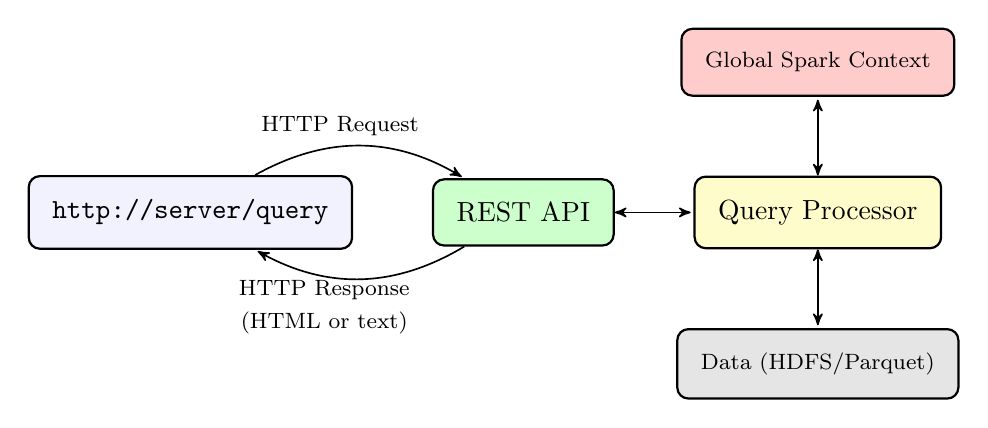
\begin{tikzpicture}
    \node[bn] (query) {{\tt http://server/query}};
    \pause

    %% \node[left=of query,align=left] () {{\bf Parameters:}\\ Date Range\\Spark Tuning Options};
    %% \pause

    \node[greenn,right=of query] (spray) {REST API};
    \node at (1.9cm,1.1cm) {{\footnotesize HTTP Request}};
    \node at (1.7cm,-1.2cm)
      {{\footnotesize HTTP Response}\\{\footnotesize (HTML or text)}};
    \draw[to] (query) edge [bend left] (spray);
    \draw[to] (spray) edge [bend left] (query);
    \pause

    \node[yn,right=of spray] (queryservice) {Query Processor};
    \draw[tofrom] (spray) -- (queryservice);
    \pause

    \node[rn,above=of queryservice] (sc)
      {{\footnotesize Global Spark Context}};
    \draw[tofrom] (queryservice) -- (sc);
    \pause

    \node[grayn,below=of queryservice] (db)
      {{\footnotesize Data (HDFS/Parquet)}};
    \draw[tofrom] (queryservice) -- (db);
  \end{tikzpicture}
  }
  \end{center}
}

\subsection{Features.}
\frame{\frametitle{\insertsection}\framesubtitle{\insertsubsection}
  \begin{itemize}
  \item<+-> Data format challenges:
    \begin{itemize}
    \item<+-> Operates on archival data with 250 columns.
    \item<+-> Data is sparse and queries use <10 columns at a time.
    \end{itemize}
  \item<+-> Use columnar data format on distributed filesystem.
  \item<+-> Spindle makes tuning parameters easy.
    \begin{itemize}
    \item<+-> Intermediate data partitioning
    \item<+-> Caching
    \end{itemize}
  \end{itemize}
}


\subsection{Queries.}
\newcommand{\nameMapsRow}[2]{#2 & #1 \\}
\newcommand{\mt}{\ensuremath{\times}}
\frame{\frametitle{\insertsection}\framesubtitle{\insertsubsection}
  \begin{itemize}
  \item Experimental setup: Representative set of analytics queries.
  \end{itemize}
  \pause
  \bigskip
\begin{table}[hb]
  \centering
  \scriptsize
  \begin{tabular}{rl}
    Shorthand & Name \\ \hline
    \nameMapsRow{Pageviews}{Q0}
    \nameMapsRow{Revenue}{Q1}
    \nameMapsRow{RevenueFromTopReferringDomains}{Q2}
    \nameMapsRow{RevenueFromTopReferringDomainsFirstVisitGoogle}{Q3}
    \nameMapsRow{TopPages}{Q4}
    \nameMapsRow{TopPagesByBrowser}{Q5}
    \nameMapsRow{TopPagesByPreviousTopPages}{Q6}
    \nameMapsRow{TopReferringDomains}{Q7}
  \end{tabular}
\end{table}
}

\frame{\frametitle{\insertsection}\framesubtitle{\insertsubsection}
  \begin{itemize}
  \item Queries use a small columnar subset.
  \end{itemize}
  \pause\bigskip
\begin{table}[ht]
  \centering
  \scriptsize
  \begin{tabular}{cccccccccc}
  & &
    Q0 &  Q1  &  Q2  &  Q3  &  Q4  &  Q5  &  Q6  &  Q7  \\ \hline
  \parbox[t]{2mm}{\multirow{11}{*}{\rotatebox[origin=c]{90}{Columns}}}
  & post\_pagename &
   \mt &      &      &      &  \mt &  \mt &  \mt &      \\
  & user\_agent &
       &      &      &      &      &  \mt &      &      \\
  & visit\_referrer &
       &      &  \mt &  \mt &      &      &      &      \\
  & post\_visid\_high &
       &      &  \mt &  \mt &      &      &  \mt &  \mt \\
  & post\_visid\_low &
       &      &  \mt &  \mt &      &      &  \mt &  \mt \\
  & visit\_num &
       &      &  \mt &  \mt &      &      &  \mt &  \mt \\
  & visit\_referrer &
       &      &      &      &      &      &      &  \mt \\
  & hit\_time\_gmt &
       &      &      &      &      &      &  \mt &      \\
  & post\_purchaseid &
       &  \mt &  \mt &  \mt &      &      &      &      \\
  & post\_product\_list &
       &  \mt &  \mt &  \mt &      &      &      &      \\
  & first\_hit\_referrer &
       &      &      &  \mt &      &      &      &      \\
  \end{tabular}
\end{table}
}

\section{Empirical Results}
\frame{\tableofcontents[currentsection]}
\subsection{Caching.}
\frame{\frametitle{\insertsection}\framesubtitle{\insertsubsection}
  \begin{itemize}
    \item<+-> Six cluster nodes (32 GB memory each), Spark and HDFS on each.
    \item<+-> 13.1GB of data, 1 week, 1 customer.
    \item<+-> {\bf Question:} How does caching in-memory improve performance?
  \end{itemize}
}

\frame{
  \centering
  \begin{tikzpicture}[every node/.style={anchor=south west}]
    \node at (0,0)(){\includegraphics[width=1\textwidth]{results-2014.08.02/caching/caching.pdf}};
    \fill[white] (1.4,0.95) rectangle (10,6) {};
    \fill[white] (6,6) rectangle (9,7) {};
    \pause
    \node at (0,0)(){\includegraphics[width=1\textwidth]{results-2014.08.02/caching/caching.pdf}};
    \pause
  \end{tikzpicture}
  \begin{itemize}
  \item<+-> Caching helps, but what else can be done to
  lower query execution times?
  \end{itemize}
}

\subsection{Data partitioning.}
\frame{\frametitle{\insertsection}\framesubtitle{\insertsubsection}
  \begin{itemize}
  \item<+-> Partitions are groups of data executed in a batch.
  \item<+-> Partitions can be executed concurrently.
  \item<+-> Not clear how to partition the intermediate data.
    \begin{itemize}
    \item<+-> Too small: Partition management overhead.
    \item<+-> Too large: Data is processed in serial.
    \end{itemize}
  \end{itemize}
}
\frame{
  \centering
  \begin{tikzpicture}[every node/.style={anchor=south west}]
    \node at (0,0)(){\includegraphics[width=1\textwidth]{results-2014.08.02/partitions/pdf/TopPages.pdf}};
    \fill[white] (1.4,0.95) rectangle (10,7) {};
    \pause
    \node at (0,0)(){\includegraphics[width=1\textwidth]{results-2014.08.02/partitions/pdf/TopPages.pdf}};
  \end{tikzpicture}
  \begin{itemize}
  \item<+-> Targeting 1.5M items in each partition is reasonable.
  \end{itemize}
}


\subsection{Benchmarking concurrent queries.}
\frame{\frametitle{\insertsection}\framesubtitle{\insertsubsection}
  \begin{itemize}
    %\item<+-> Multiple users can utilize an analytics system like SiteCatalyst
    %  concurrently, and Spark can be used in multithreaded applications.
    \item<+-> How much will Spindle's performance
      degrade if multiple users are utilizing it at the same time?
    \item<+-> Concurrently call the same query on the same data.
    \item<+-> Average execution times.
    %\item<+-> {\bf Solution:} Assume users submit the same query
    %  at the same time and observe the average query response time.
    %% \item<+-> A Python script using threading manages threads for
    %%   each number of concurrent queries.
    %% \item<+-> Consider the example below for 2 threads and 3 repeated
    %%   queries per thread. The first thread finishes before the second,
    %%   and remains loaded until the second thread finishes.
    %%   $t_4^1$ and $t_5^1$ are not used in the average.
    %% \item<+-> This experiment runs queries on the date range of
    %%   Jan 1, 2014 to Jan 7, 2014 and each thread calls the query 4 times.
  \end{itemize}
}

\newcommand{\revealConcurrent}[1]{
  \frame{
    \begin{tikzpicture}[every node/.style={anchor=south west}]
      \node at (0,0)(){\includegraphics[width=\textwidth]{#1}};
      \fill[white] (1.5,0.95) rectangle (10,6.8) {};
      \pause
      \node at (0,0)(){\includegraphics[width=\textwidth]{#1}};
    \end{tikzpicture}
    \begin{itemize}
    \item<+-> Performance better than serializing concurrent
      requests, but can be improved.
    \end{itemize}
  }
}
%% \revealConcurrent{results-2014.08.02/concurrent/pdf/TopPages.pdf}
\revealConcurrent{results-2014.08.02/concurrent/pdf/TopPagesByPreviousTopPages.pdf}

\subsection{Scaling Spark and HDFS workers.}
\frame{
  \centering
  \begin{tikzpicture}[every node/.style={anchor=south west}]
    \node at (0,0)(){\includegraphics[width=1\textwidth]{images/scalingWorkers.pdf}};
    \fill[white] (2,0.95) rectangle (7.3,6) {};
    \pause
    \node at (0,0)(){\includegraphics[width=1\textwidth]{images/scalingWorkers.pdf}};
  \end{tikzpicture}
  \begin{itemize}
  \item<+-> Further profiling is needed to improve performance as
    increasing the number of workers.
  \end{itemize}
}

\section{Future Work}
\frame{\tableofcontents[currentsection]}
\frame{\frametitle{\insertsection}\framesubtitle{\insertsubsection}
  \begin{itemize}
  \item<+-> Lowering query execution time.
    \begin{itemize}
    \item<+-> Goal: Sub-second.
    \end{itemize}
  \item<+-> Automatically tuning parameter exploration space for
    a given workload.
    \begin{itemize}
    \item<+-> Online/Dynamically
    \item<+-> Offline
    \end{itemize}
  \item<+-> Results caching for exact same queries.
  \item<+-> Data preprocessing to remove redundant computations.
  \end{itemize}
}

\section{Conclusions}
\frame{\tableofcontents[currentsection]}
\frame{\frametitle{\insertsection}\framesubtitle{\insertsubsection}
  \begin{itemize}
    %\item<+-> Spark is a good candidate for expressing web analytics queries.
  \item<+-> We present {\bf Spindle}.
      \begin{itemize}
      \item<+-> {\bf Open-source} prototype analytics processing engine.
      \item<+-> Sample set of web analytics queries.
      \item<+-> Interface for parameter tuning.
      \end{itemize}
  \end{itemize}
  \pause
  \vspace{4mm}
  \begin{center}
    {\scriptsize
      \begin{tabular}{r|l}
      Spindle Project & \url{http://github.com/adobe-research/spindle} \\
      Demo & \url{http://adobe-research.github.io/spindle/} \\
      Brandon Amos & \url{http://github.com/bamos} \\
      David Tompkins & \url{http://github.com/DavidTompkins} \\
      \end{tabular}
    }
  \end{center}
}

\end{document}
